%!TEX root = ../Thesis.tex

\def\chapdir{./ChapterPerception}

\chapter{Algorithm Solution}\label{ch:perception}

%%%%%%%%%%%%%%%%%%%% Introduction %%%%%%%%%%%%%%%%%%%
Following the literature, the two main options for increasing the accuracy is extensive modelling of the errors, or some type of differencing algorithm. Error modelling requires external hardware, internet connection and extra computation time which increases the budget requirements.\\

The common theme throughout the literature is to use differencing to minimise errors, both through time and space. For a single receiver differencing through space, a second known location is still required. This is set up externally and services a set area. However for multiple receivers, spacial differencing is available. Even though with multiple receivers there is the added pre-processing with the sending of data between nodes and computation for epoch alignment. When differencing through time, the epoch alignment is required at the receiver end. That is, to manipulate the measurements as if the receivers took readings at the same time. Depending on how precise the alignment required for a system is, the computation time may require a numerical iteration solution. Using multiple receivers and only differencing through space, the epoch alignment must be at the satellite end, so that the signal has the same start point to precisely calculate the spatial difference.



\section{Proposed Planar Algorithm (PA)}
This new algorithm is derived from taking the difference in pseudorange between multiple receivers from one satellite and expressing the distances as planes.

\begin{figure}[h]
\centering
\caption{2D representation}
\label{fig:overall_singleS_multiR}
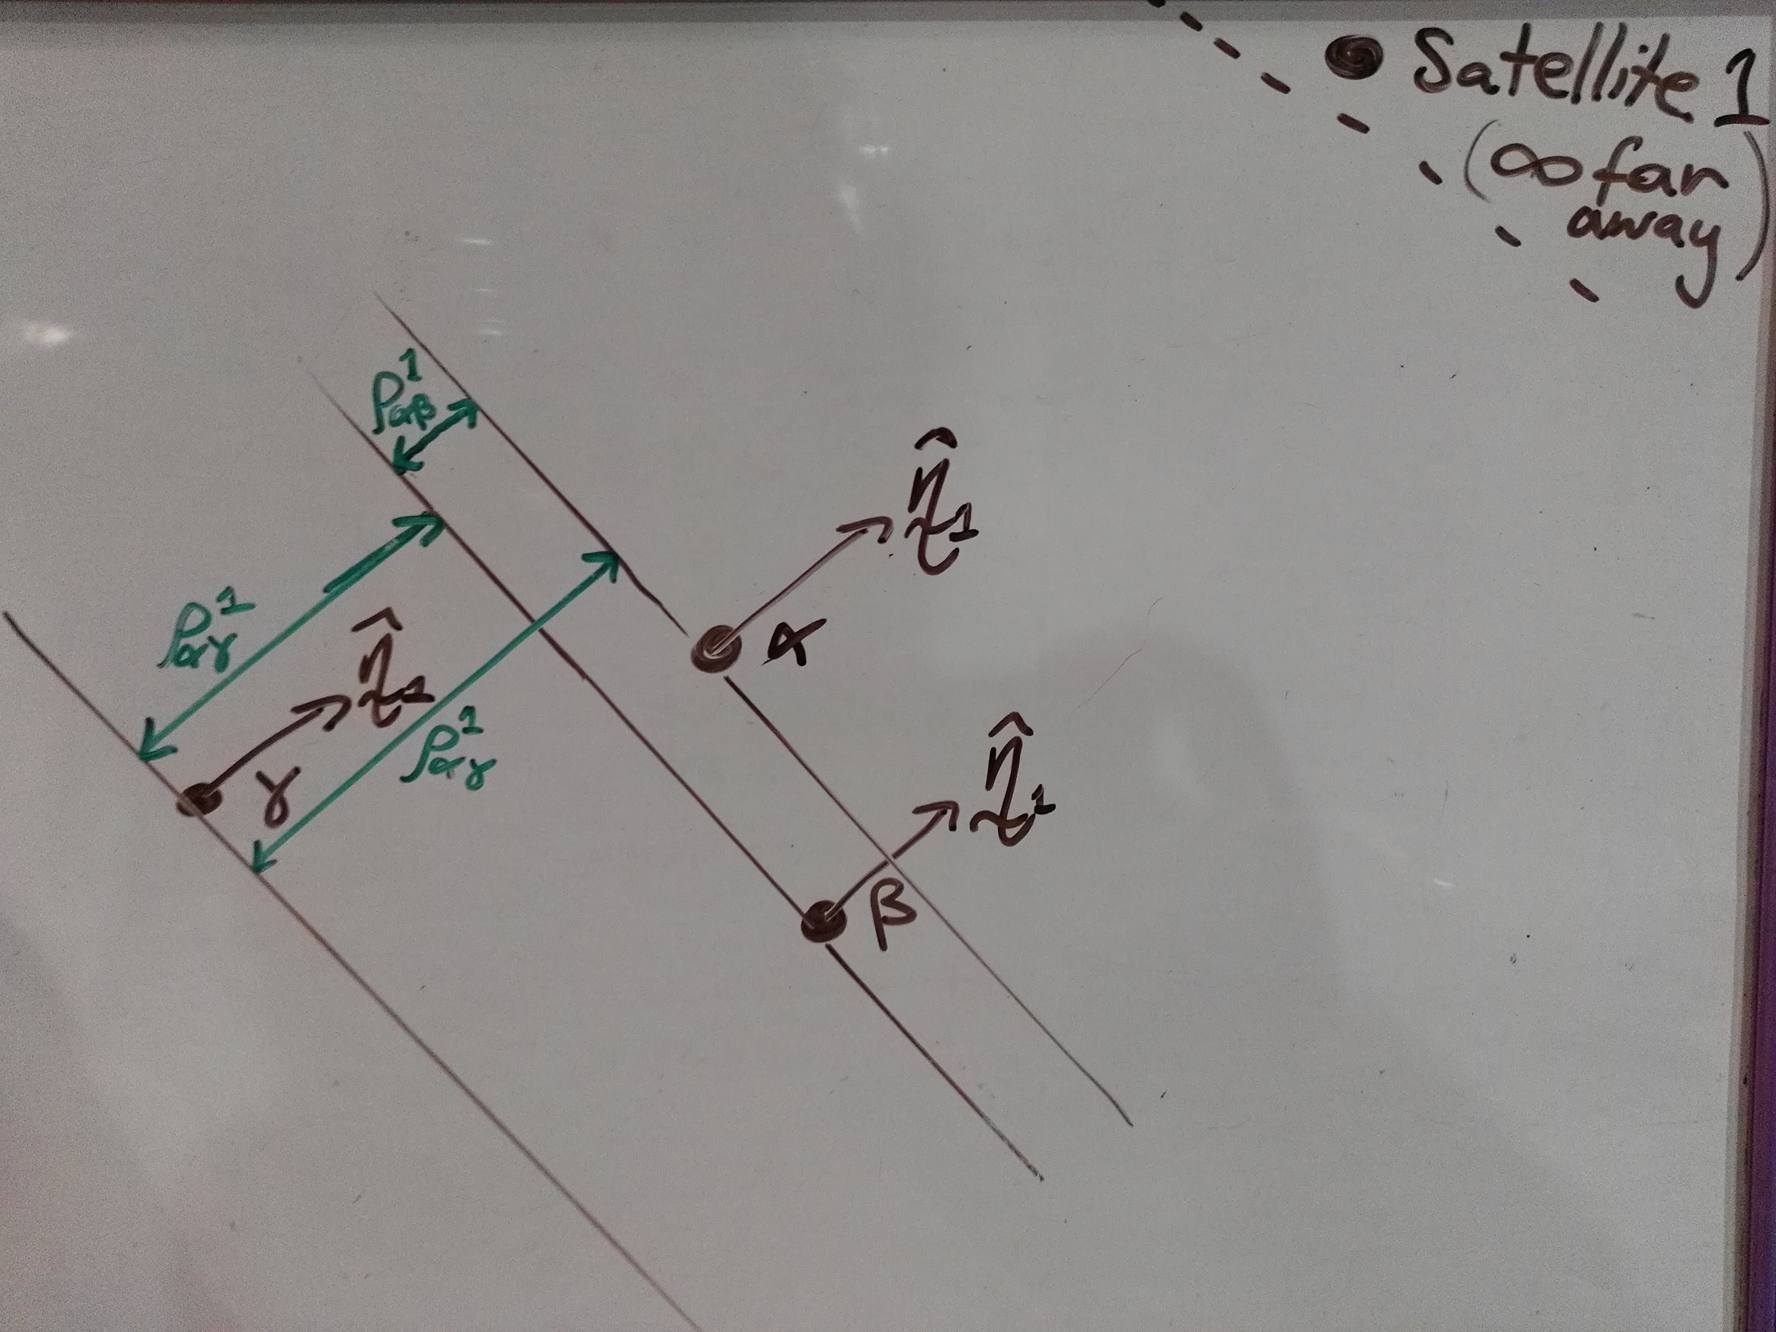
\includegraphics[width=0.7\linewidth]{ChapterLiteratureReview/overall_singleS_multiR.jpg}
\end{figure}

With multiple satellites in view, the intersection of planes for a particular receiver is the position of the receiver.
\begin{figure}[h]
\centering
\caption{}
\label{fig:overall_multiS_duelR}
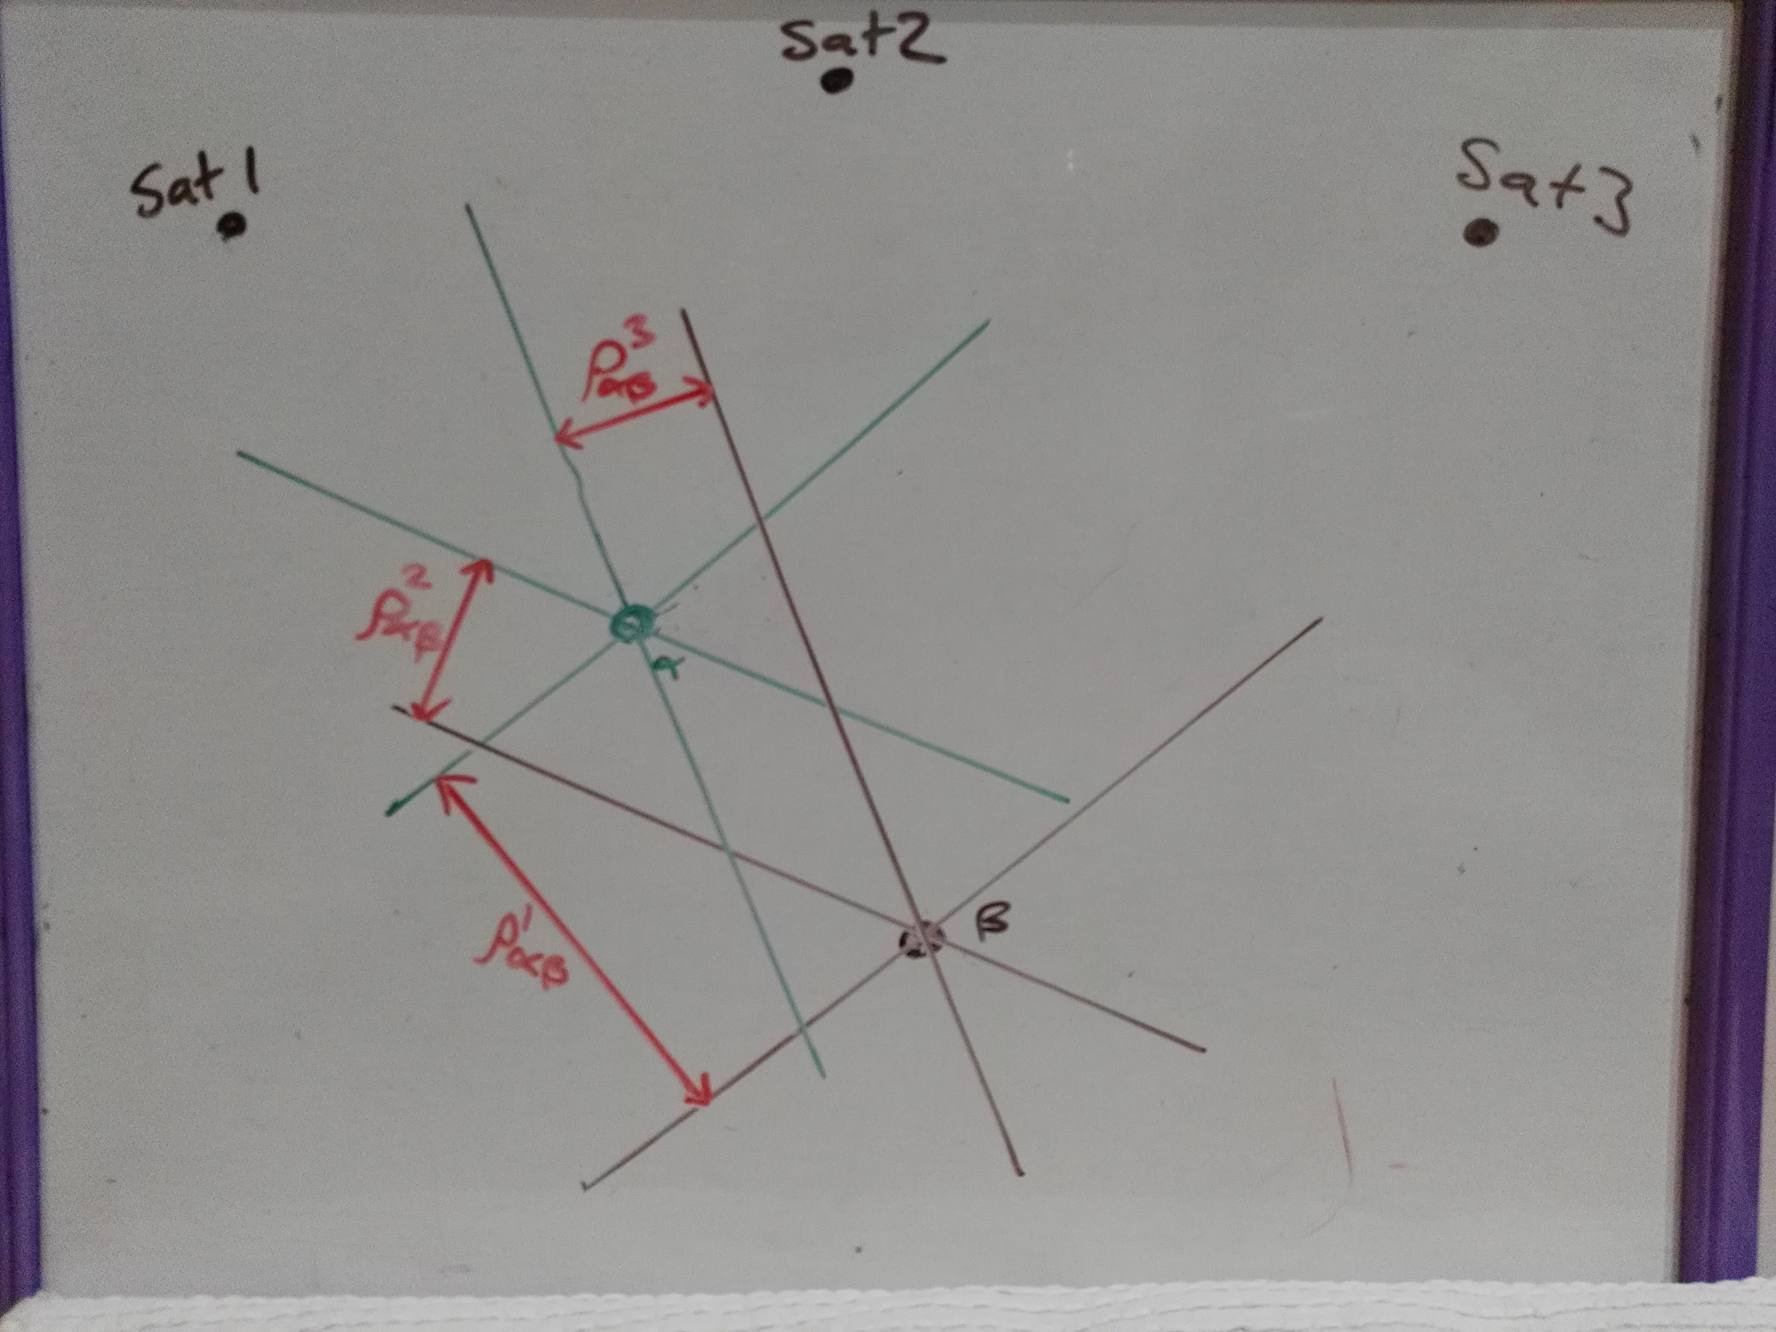
\includegraphics[width=0.7\linewidth]{ChapterLiteratureReview/overall_multiS_duelR.jpg}
\end{figure}

With this strategy, some of the errors that plague the absolute position are negated for the relative position. Eq\eqref{Eq:full} describes the measured pseudorange for a single receiver $\omega$ from a single satellite $s$.
\begin{eqnarray}
\rho_\omega^s = R_\omega^s -cb_\omega + c(T_s + I_s+\nu_s+b_s) + \epsilon \label{Eq:full}
\end{eqnarray}
Where $R_\omega^s$ is the real range with the following sources of error; $b_\omega$ is the receiver clock bias, $T_s$ is the tropospheric error, $I_s$ is the ionospheric error, $\nu_s$ is the relativistic error, $b_s$ is the satellite clock bias and $\epsilon$ is random noise. The satellite correlated effects are removed with the individual receiver clock biases, random error and true range difference, Eq\eqref{Eq: D}.  
\begin{eqnarray}
D_{\omega_i\omega_j}^s &=& \rho_{\omega_i}^s - \rho_{\omega_j}^s \\
D_{\omega_i\omega_j}^s &=& R_{\omega_i}^s-R_{\omega_j}^s -c(b_{\omega_i}-b_{\omega_j}) + \epsilon \label{Eq: D}
\end{eqnarray}

This chapter explains the assumptions and details the methodology behind the planar algorithm.





%%%%%%%%%%%%%%%%%%%% Content Sections %%%%%%%%%%%%%%%%%%%

%!TEX root = ../Thesis.tex

\section{Assumptions}
All the assumptions are based on each other so need a pre-statement

\subsection{Approximate Global Location}
An approximate location is required for where the system is on the Earth within 1 km of all of the receivers. This is to calculate the normal direction vectors to each of the satellites. A simple solution to this is to set the reference receiver to calculate it's absolute position first using NLLS. This will give the system a reference of within 20 m at worst, well within the acceptable parameters.


\subsection{Static Receivers}
All receivers are assumed to be static for the time in between all receivers to get a sample reading. This makes for an easier transform to align the satellite positions to a common epoch. It also ignores the problem of how the pseudorange from each receiver would be sent to either all of the receivers or to a central device for computation and the time delay associated with that. \\

For the dynamic case, it is likely that the data would be a part of a system containing other signals that describe the motion such as dead reckoning. In that case, the location of the receiver at the common epoch time can be back calculated to minimise the dynamic error. The incorporation of moving receivers is an area to explore for future work on the algorithm. However, there are existing algorithms in the literature XX where the relative motion is tracked with sub meter accuracy that may be more appropriate for complex dynamic systems.


\subsection{Parallel plane assumption}
It as assumed for the plane equations that all receivers point to a satellite along the same vector. This is valid for a dispersion of receivers for 10km for an error of XX. This is synonymous to if the satellites were at infinity and all the receiver vectors are parallel to a satellite


\begin{eqnarray}
\delta &=& \tan^{-1}\left(\frac{d}{a}\right) \label{Eq:parplane delta}\\
e &=& 2d\tan\delta \label{Eq: parplane e(d)}\\
\eqref{Eq:parplane delta} \& \eqref{Eq: parplane e(d)}\Rightarrow e&=&\frac{2d^2}{a} \label{Eq:squarerel}
\end{eqnarray}
Where a is the altitude, d is the distance between two receivers and e is the error in the plane created. The worst configuration for error in the vector normal to the plane is if the satellite is directly above the receivers at the smallest distance from the Earth in orbit, $a>20000\;km$. For d=5 km the perpendicular error is 2.5 m





%!TEX root = ../Thesis.tex

\section{Epoch Alignment} \label{sec:epochalignment}

A single sample of pseudoranges from any two receivers will not be taken at the exact same time without a connecting network to implement control. This increases the setup requirements which in turn increases the cost of the system and reduces the ease of compatibility with different receivers. The earliest time between all the receivers will be used as the time reference point called common epoch. The satellite position in the future time steps were backcalculated to find the difference in the pseudorange. The time between receivers would be a maximum of one second, as the slowest sampling time is typically 1 Hz. This extra distance is only in the vacuum of space and is not affected by potential nonlinear affects such as ionosphere and troposphere errors that affect the speed of light.\\

The known variables from the raw GPS data is the time the sample measurement was taken $t_\omega$ and the pseudorange to each visible satellite $\rho_\omega^1$ for each receiver $\omega$.

By the distributive law, Eq\eqref{Eq: epochdist} mathematically describes the vector relationship in Figure \ref{Fig:epochsync}.
\begin{eqnarray}
\hat{\eta}\cdot s + \hat{\eta}\cdot v = |\eta|  \label{Eq: epochdist}
\end{eqnarray}
The vector $s$ is the transform of the satellite from time $t_2$ to the common epoch time $t_1$. It is extracted from the navigation message of the signals.

The vector $v$ is the measured pseudorange of a receiver from a particular visible satellite at $t_2$ with an unknown direction vector. The direction vector is unknown because the position of the receiver is what is being solved for. The vector $\eta$ describes the known direction vector from the single approximate location of the geographic region to the common epoch of a particular visible satellite. It is the magnitude of $\eta$ that describes what the pseudorange would have been if the measurement was taken at the common epoch. The difference between $|\eta|-|v|$ is the correction term $\Delta\rho$, see Eq \eqref{Eq:deltarho}.
\begin{eqnarray}
\Delta \rho &=& |\eta| - |v|\\ % check -ves
\Delta \rho&=& \hat{\eta}\cdot s + \hat{\eta}\cdot v - |v|\\
\Delta \rho&=& \hat{\eta}\cdot s + |\hat{\eta}||v|\cos(\theta) - |v| \label{Eq:deltarho}
\end{eqnarray}
As |v| is >20 000 km and s is <4 km (as the maximum time between signals is 1 seconds), $\theta\approx 0$ which means $\cos\theta\approx1$. The magnitude of a unit vector is one therefore: \eqref{Eq:deltarho} simplifies to:
\begin{eqnarray}
\Delta\rho = \hat{\eta}\cdot s 
\end{eqnarray}
Because of the asynchronous time, some of the satellite correlated errors would not correlate as well as if it was from the same point in time. This is because the path through the ionosphere and troposphere is not exactly the same. 
\begin{figure}[h]
\centering
\caption{Vector Epoch Synchronisation}
\label{Fig:epochsync}
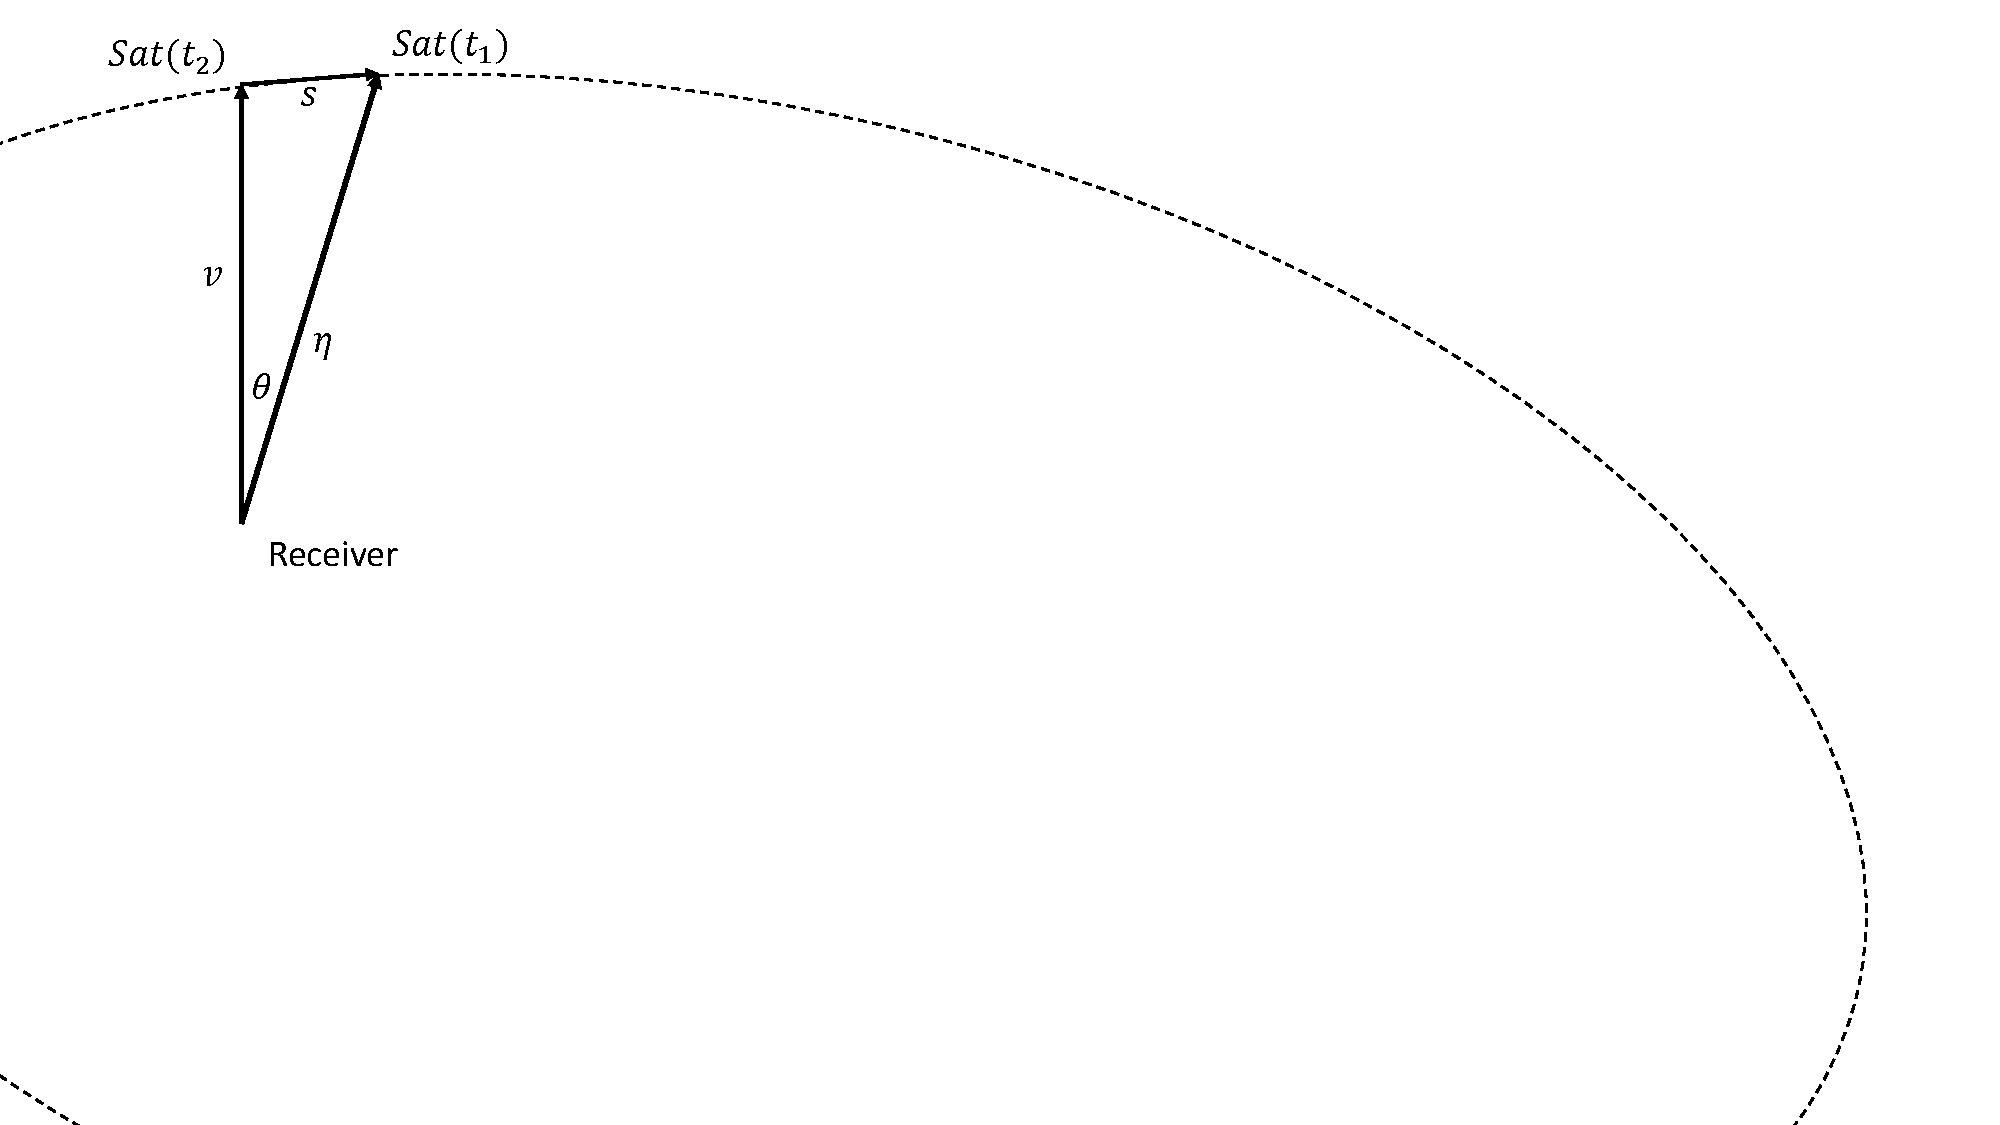
\includegraphics[trim=0 10cm 23cm 0,clip,width=0.3\linewidth]{ChapterPerception/Figures/epochalignment.pdf}
\end{figure}

% type up maths for this assumption- thats it - not an assuption, this goes into the algorithm- assumption is the asynch time described by (sample offset-time of flight) has error in position of satellite as there is error in time of flight - or do you know position of sat when sent????????









%!TEX root = ../Thesis.tex
\section{Planar Intersection Algorithm}

- assume satellite is at infinity for comparing difference in pseudorange for a particular reference satellite.\\
- use all satellites as reference satellite - no single point of failure, also not all satellites might be in view for all receivers\\
- get the normal vector between all receivers and each sat. \\
- Calculate the average normal vector.\\
- get the difference in pseudorange between all receivers along each normal vector \\
- create a plane with the normal vector with that distance\\
- solve via optimization (least squares) \\
- use clock adjustment from abs gps? or have as another optimisation variable\\
- antenna problems? misalignment?\\
- share clock bias's between solving for different reference sets? - do it one by one or all together?\\
- need to align the time of signal sent to the receivers before calculating average normal vector\\

- have weighted planes based on ? have weighted area on the planes?\\
- if one plane intercepts far away from the others then ignore it (multipath). hyperdimensional surface to minimise




% conceptual
how to send data between receivers? do it offline on a different platform?


https://www.e-education.psu.edu/geog862/node/1759 - errors in pseduorange

http://www.insidegnss.com/node/2898 - how to get pseudorange from raw data




\subsection{Algorithm}

\subsubsection{Pre-Processing}
\paragraph{Select reference receiver $\alpha$}
The receiver $\alpha$ is used as the reference location and common time in the NED frame. 
\paragraph{Collect data of one timestep from all receivers}
The raw data as well as the estimated absolute location and clock bias (what frame of reference is this?) from non-linear least squares optimisation is collected from all GNSS receivers.
\paragraph{Align to reference Epoch time}\label{timetransform}


\subsubsection{Distance Optimisation}
By optimising the distance between each pair of receivers, the error in the whole system is minimised. 
This means that the position receivers are not only relative to the reference receiver $\alpha$ but between all receivers just with the reference frame origin located at $\alpha$. It is because of this step a receiver does not need to have all the same satellites in view as all other receivers, including the designated $\alpha$.


\paragraph{Average normal Vector}
Find the average normal vector pointing to each satellite $\hat{\eta_s}$ from the receivers. The normal vector is calculated by using the position all of the satellites in view at the common time $t_{\alpha}$ as previously transformed in \ref{timetransform} and the estimated absolute position of all receivers. The average for each satellite is calculated by taking the mean across all receivers.

\paragraph{Difference in Pseudorange}
The differences in pseudorange are calculated $\Delta\rho^s_{\omega_i\omega_j}$ where s is the satellite, $\omega_i$ and $\omega_j$ are receivers $(for i<j, i\neq j)$. 

\paragraph{Optimise Pseudorange}
The pseudorange between each pair of receivers along each normal vector $\hat{\eta_s}$ creates an overdetermined linear system that is solved via least squares.
\begin{figure}
\centering
\caption{text}
\label{key}
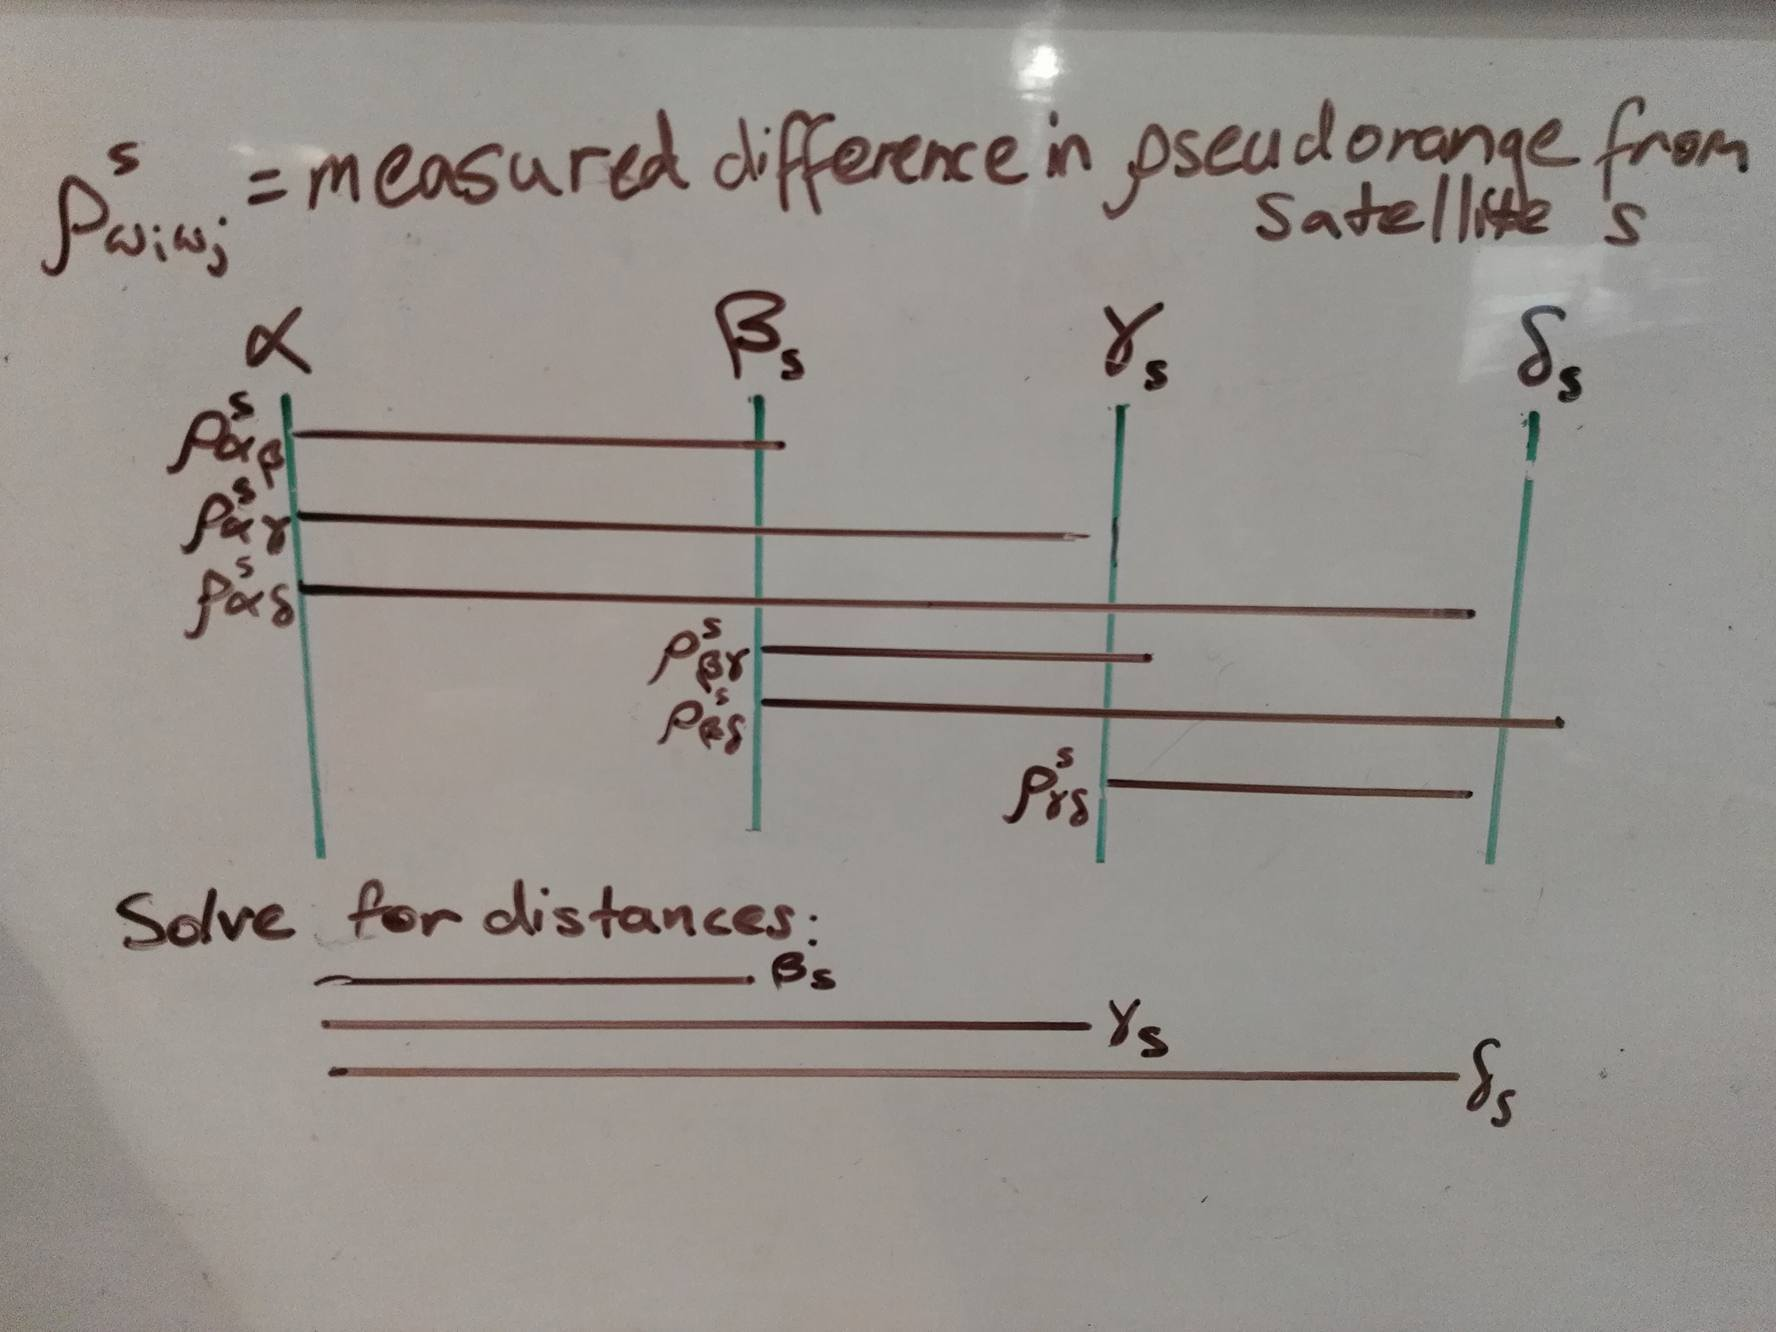
\includegraphics[width=0.7\linewidth]{ChapterPerception/Figures/solve_distances.jpg}
\end{figure}
\begin{eqnarray}
\Phi &=& \begin{bmatrix}
0 & -1 & 0 & ...\\
0 & 0 & -1 & ...\\
... & ... & ... & ... \\
1 & -1 & 0 & ...\\
1 & 0 & -1 & ...\\
\hdotsfor{4} \\
0 & 1 & -1 & ...
\end{bmatrix} \\
%
\Omega_s &=& \begin{bmatrix}
\beta_s \\
\gamma_s\\
\delta_s \\
\vdots
\end{bmatrix} \\
%
\rho_s &=& \begin{bmatrix}
\rho_{\alpha\omega_1}\\
\rho_{\alpha\omega_2}\\
\hdotsfor{1}\\
\rho_{\omega_1\omega_2}\\
\rho_{\omega_1\omega_3}\\
\vdots
\end{bmatrix} 
\end{eqnarray}

\begin{eqnarray}
\Phi\times\Omega_s = \rho_s
\end{eqnarray}
Solve by linear least squares for an overdetermined system by the pseudo inverse matrix
\begin{eqnarray}
\Omega_s = (\Phi^T\Phi)^{-1}\Phi^T\rho_s
\end{eqnarray}

\subsubsection{Point Optimisation}
\paragraph{Create Planes}
Create sets of planes for each receiver $\omega$ from the normal vectors $\hat{\eta_s}$ and the set of distances from the reference point $\alpha$ to receiver $\omega$ along each of the normal vectors denoted $\Omega_\omega$.

The equation of a plane is $Ax+By+Cz+D=0$ where the coefficients [A,B,C] describe the normal vector of the plane and the coefficient D sets the plane in 3D space along the vector. As the normal vector is already calculated for each satellite, only the D coefficient must be solved for each receiver and satellite pair. 
\begin{eqnarray}
P_\omega^s &=& (i\cdot\hat{\eta_s})x + (j\cdot\hat{\eta_s})y + (k\cdot\hat{\eta_s})z + D_\omega^s \label{genplane}\\
P_\omega^s &=& I\cdot H +D_\omega\\
\end{eqnarray}
Where $I = x\hat{\textbf{i}}+y\hat{\textbf{j}}+z\hat{\textbf{k}}$ is the *identity* vector and H is a matrix of normal vectors to each satellite:
\begin{eqnarray}
H = \begin{bmatrix}
\hat{\eta_1} \\
\hat{\eta_2} \\
\vdots\\
\hat{\eta_n}
\end{bmatrix}
\end{eqnarray}
The coefficient D can be calculated by finding a point on the plane $f_\omega^s$, then substituting it into \eqref{genplane} for x,y,z. The point of the plane is calculated by moving along the normal vector by the optimised pseudo distance from the reference point \eqref{Eq:f}.
\begin{eqnarray}
f_\omega^s &=& \Delta_\omega^s\hat{\eta_s} \label{Eq:f}\\
P_\omega^s &=& \hat{\eta_s}\cdot f_\omega^s +D_\omega^s = 0\\
D_\omega^s &=& -\hat{\eta_s}\cdot f_\omega^s\\
D_\omega^s &=& -\Delta_\omega^s ||\hat{\eta_s}|| \\
||\hat{\eta_s}|| &=& 1\\
D_\omega^s &=& -\Delta_\omega^s\\
\Rightarrow P_\omega^s &=& I\cdot H -\Omega_\omega
\end{eqnarray}

\begin{figure}[h]
\centering
\caption{Find position $f_\omega^s$ on the plane}
\label{fig:pointonplane}
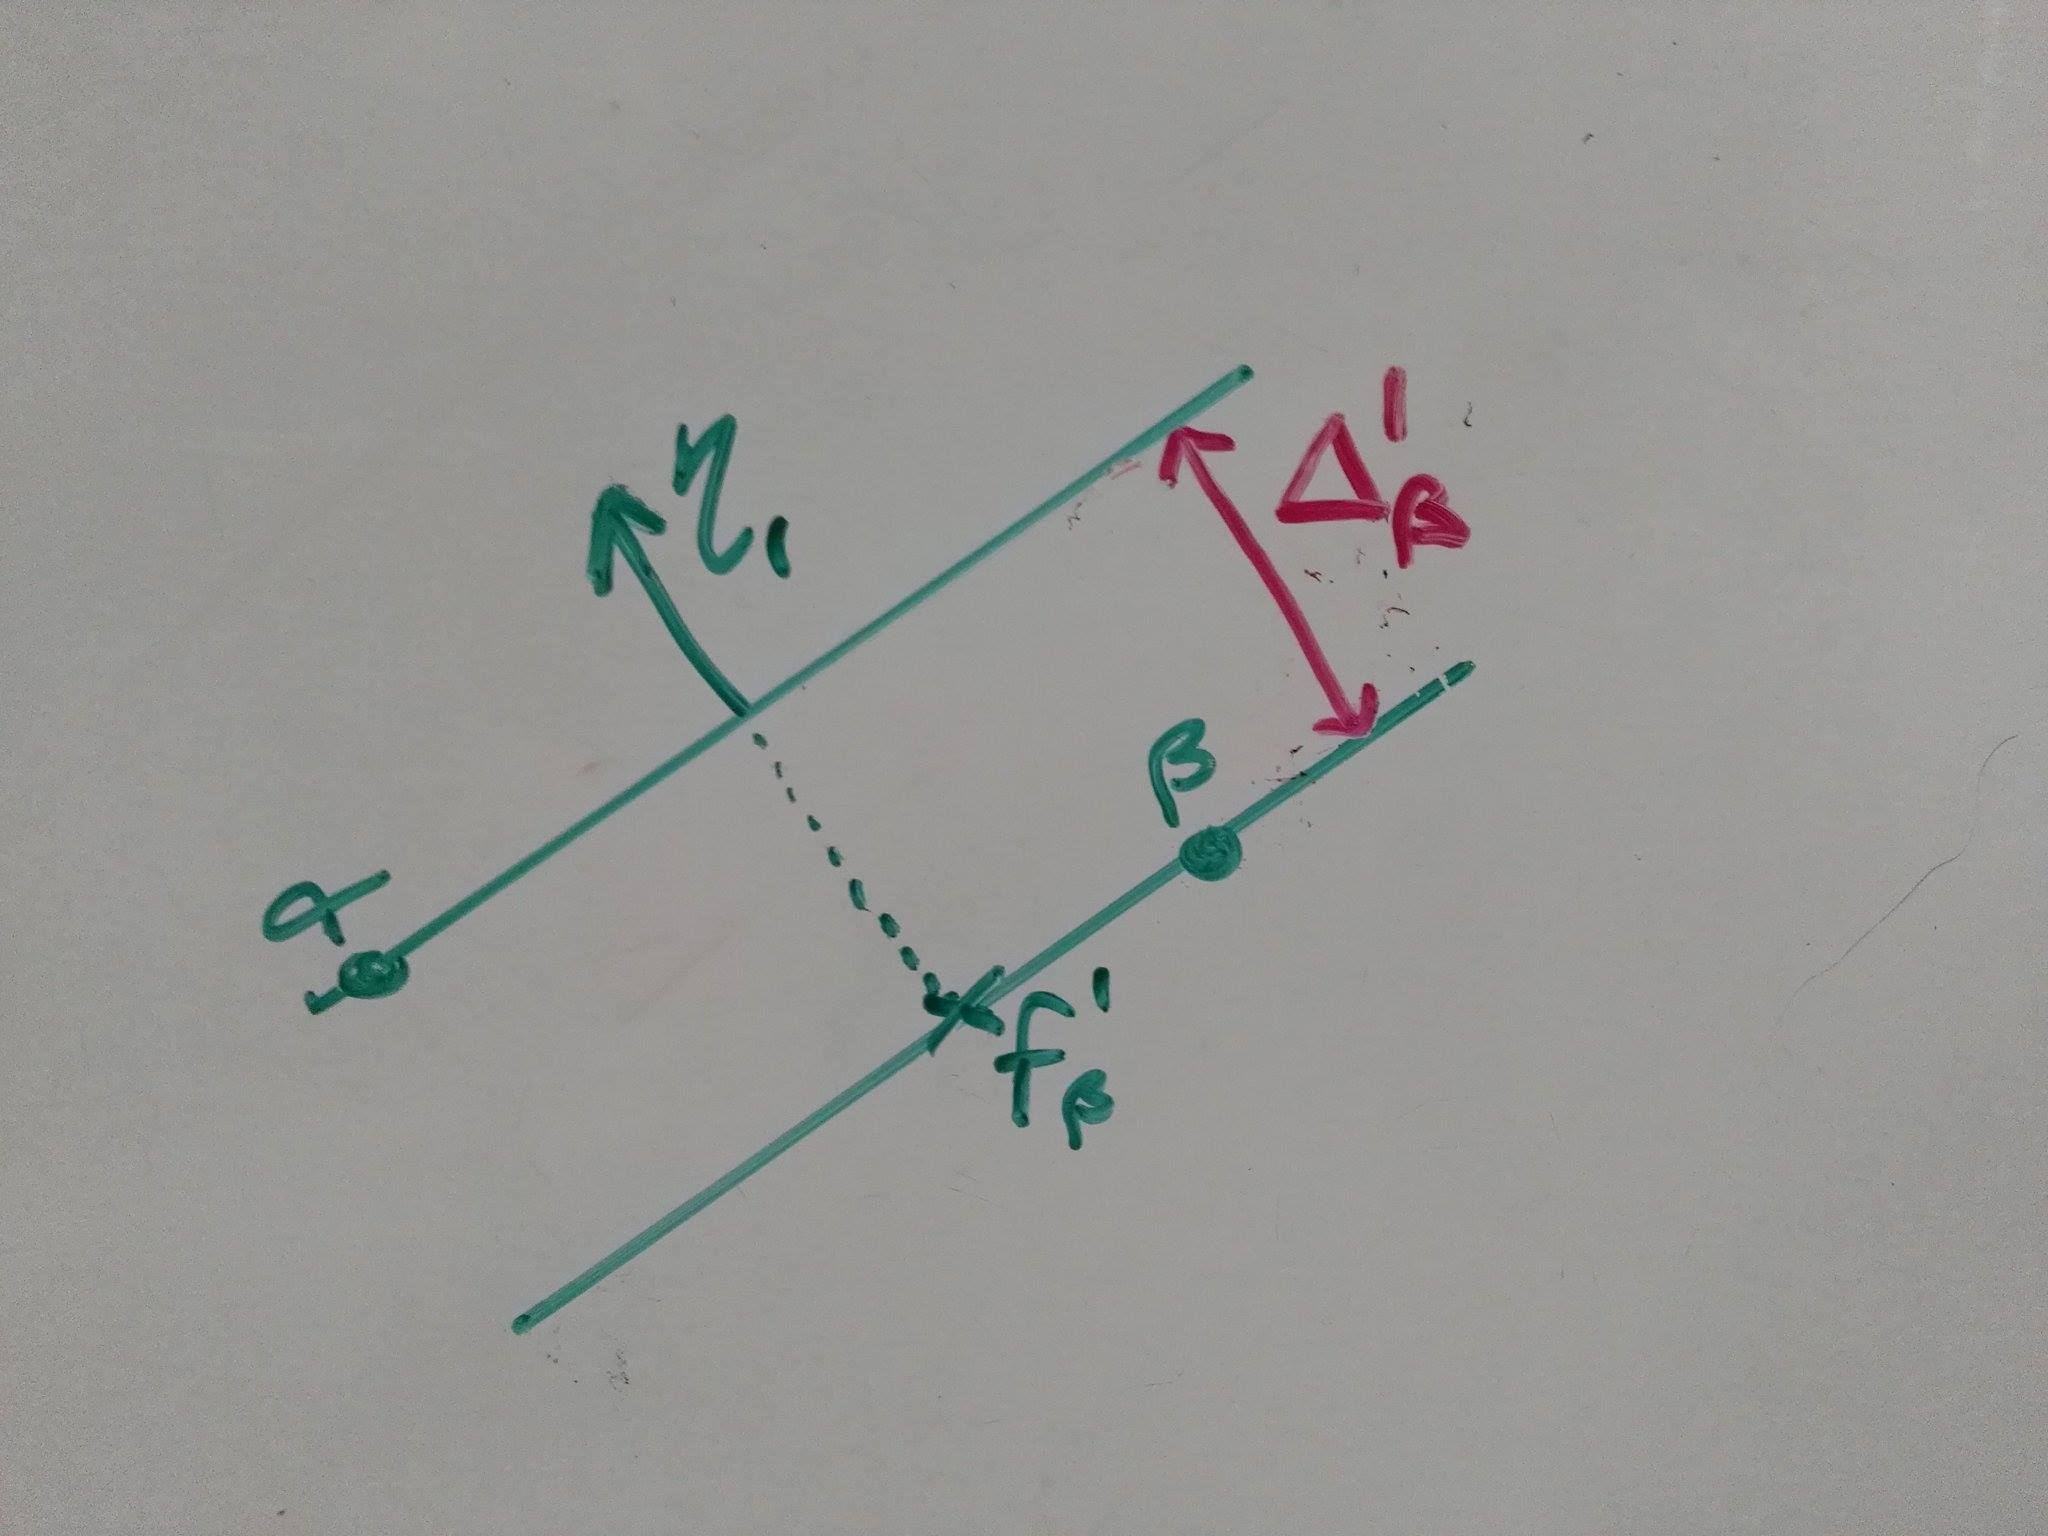
\includegraphics[width=0.7\linewidth]{ChapterPerception/Figures/pointonplane}
\end{figure}






$\Omega_\omega$ is a vector of optimised pseudo-distances from reference $\alpha$ to receiver $\omega$ for all satellites $s\in{1,2...n}$
\begin{eqnarray}
\Omega_\omega = \begin{bmatrix}
\Delta_{\omega}^1 \\
\Delta_{\omega}^2 \\
\vdots\\
\Delta_{\omega}^n \\
\end{bmatrix}
\end{eqnarray}
Where $\Omega_s$ is the vector of optimised pseudo-distances from $\alpha$ to each receiver $\omega\in1,2...m$ for a single satellite s:
\begin{eqnarray}
\Omega_s = \begin{bmatrix}
\Delta_{\omega_1}^s \\
\Delta_{\omega_2}^s \\
\vdots\\
\Delta_{\omega_m}^s \\
\end{bmatrix}
\end{eqnarray}


\paragraph{Solve for Intersection}
As the system of homogeneous linear equations is overdetermined, it can be solved using singular value decomposition to find a point that has the minimum residuals from all of the planes in its set $P_\omega$. Each set of planes for a particular receiver is independent to all other receivers. The vector $X_\omega$ describes the position of receiver $\omega$ in NED coordinates and $\tau_\omega$ describes a final receiver clock bias that alters the displacement of all the planes in the set $P_\omega$ by the same parameter.
\begin{eqnarray}
X_\omega &=& \begin{bmatrix}
x_\omega \\y_\omega \\ z_\omega \\ \tau_\omega
\end{bmatrix}\\
P_\omega X_\omega &=& D_\omega \\
\end{eqnarray}
In order to solve all of the receivers with the least amount of error in the whole system, all of the position vectors $X_\omega$ are solved at the same time. The reference planes of $\alpha$ must be included as a constraint on the system. All of the clock biases are also constrained with the clock bias from $\tau_\alpha$, see \eqref{Eq: P with alphat}.
The receiver clock bias only affects the equation of the planes by altering the constant as a change in the pseudorange has no affect over the angle of the plane. Each receiver clock bias alters all the planes associated with that receiver proportionally. 
\begin{eqnarray}
P_\omega^s &=& (i\cdot\hat{\eta_s})x + (j\cdot\hat{\eta_s})y + (k\cdot\hat{\eta_s})z + D_\omega^s + (\tau_\omega-\tau_\alpha) \label{Eq: P with alphat}\\
\end{eqnarray}
 



%%%%%%%%%%%%%%%%%%%% Conclusions %%%%%%%%%%%%%%%%%%%


